% Provenance (never printed): see sources/outline_sources.md (Year 2: index minerals and zones,
% geothermometers and geobarometers, prograde and retrograde paths, metamorphic series,
% ultrahigh-pressure rocks and exhumation, ocean-floor metamorphism). Garnet-biotite
% calibration refitted from the Ferry and Spear (1978) brackets tabulated by Holdaway et al.
% (1997); GASP from Koziol and Newton (1988); thickening model after England and Thompson
% (1984) in figdata/bachelor-2/ptpaths.py; exercise and problem values in the Book 4 scratch
% calculators calc/ch11.py and calc/ch11b.py.
\chapter{तापदाबमिति और P--T--t पथ}\label{ch:b2:pt-paths}

किसी शिस्ट में उगा कुछ मिलीमीटर चौड़ा एक गार्नेट अपने क्रोड में वह संघटन रखता है
जो उसका उगना शुरू होते समय था, और अपने किनारे में वह संघटन जो उगना रुकते समय था। हर
मंडल उस समय अपने आसपास के बायोटाइट और प्लैजियोक्लेज़ के साथ साम्य में था, और
इन खनिजों के बीच लोहा, मैग्नीशियम और कैल्सियम जिस तरह बँटे, वह तापमान
और दाब पर निर्भर करता है। पिछले अध्याय के ऊष्मागतिकी के साथ पढ़ा जाए तो गार्नेट बताता है कि
उसकी चट्टान कितनी गहराई तक दबी और कितनी गर्म हुई; काल-निर्धारित होने पर वह बताता है कब, और
चट्टान कितनी तेज़ी से ऊपर लौटी। यह अध्याय कायांतरी खनिजों को तापमापी, दाबमापी
और घड़ियों में बदलता है, और भूपर्पटी में से एक चट्टान के पथ का अनुसरण करता है।

\begin{recall}
\textbf{पुस्तक 2 (उच्च माध्यमिक) से}: \omterm{def:b2:metamorphic-facies:metamorphism}{कायांतरण} श्रेणी, सूचक खनिज और समश्रेणी-रेखाएँ।
\textbf{पुस्तक 3 (स्नातक वर्ष 1) से}: जियोथर्म और रेडियोजनिक ऊष्मा-उत्पादन; लगभग
\qty{35}{km} मोटी महाद्वीपीय भूपर्पटी; रेडियोमितीय काल-निर्धारण, किसी खनिज का अवरोध-तापमान
और उससे मिलने वाली शीतलन-आयु; महासागरीय भूपर्पटी और उसका \omterm{def:b2:mantle-melting:peridotites}{पेरिडोटाइट}।
\textbf{भौतिकी की पुस्तकों से}: ऊष्मा-समीकरण $\partial T/\partial t = \kappa\,
\partial^2 T/\partial z^2$ और तापीय विसरणशीलता $\kappa$। \textbf{रसायन-विज्ञान की
पुस्तकों से}: साम्य स्थिरांक, $\Delta_r G^\circ + RT\ln K = 0$, और आदर्श विलयनों में
सक्रियताएँ। \textbf{\cref{ch:b2:metamorphic-facies} से}: कायांतरी अभिक्रियाएँ,
\omterm{def:b2:metamorphic-facies:clapeyron}{क्लेपेरॉन ढलान}, \ce{Al2SiO5} आरेख और संलक्षणियाँ।
\end{recall}
% ledger: prem:moho-average

\section{कायांतरी मंडल}\label{sec:b2:pt-paths:zones}

स्कॉटिश हाइलैंड्स के पंकाश्मों में जॉर्ज बैरो ने 1890 के दशक में मंडलों का एक अनुक्रम
मानचित्रित किया, जिनमें से हर एक किसी नए सूचक खनिज के पहली बार प्रकट होने से चिह्नित है। उच्चतर
श्रेणी की ओर जाने पर क्लोराइट के साथ क्रम से बायोटाइट, गार्नेट, स्टॉरोलाइट, कायनाइट और सिलिमेनाइट जुड़ते हैं;
प्ररूपी परिच्छेदों में गार्नेट से सिलिमेनाइट तक के मंडल लगभग 500 से
\qty{650}{\celsius} और 5 से \qty{7}{kbar} पर बने।
% ledger: iugs:barrow, barrow1893:paper, earle:regional

\begin{definition}[बैरोवियन मंडल; कायांतरी क्षेत्र-प्रवणता]\label{def:b2:pt-paths:barrovian}
\emph{बैरोवियन मंडल}\index{बैरोवियन मंडल} \omterm{def:b2:metamorphic-facies:protoliths}{मेटापेलाइटों} के वे कायांतरी मंडल हैं जो
इस क्रम में आते हैं: क्लोराइट, बायोटाइट, गार्नेट, स्टॉरोलाइट, कायनाइट, सिलिमेनाइट,
और हर एक अपने सूचक खनिज की समश्रेणी-रेखा से शुरू होता है। किसी प्रदेश
की \emph{कायांतरी क्षेत्र-प्रवणता}\index{कायांतरी क्षेत्र-प्रवणता}
दाब--तापमान तल में वह वक्र है जो उसकी चट्टानों द्वारा अंकित
शिखर-दशाओं से होकर जाता है, उन स्थानों पर जहाँ वे आज अनावृत हैं।
\end{definition}

क्षेत्र-प्रवणता का हर बिंदु एक अलग चट्टान से आता है, और हर चट्टान अपने शिखर पर
अपने समय पर पहुँची: क्षेत्र-प्रवणता न तो किसी एक क्षण का जियोथर्म है, न ही
किसी एक चट्टान का पथ। यह वह छाप है जो शिखर वर्तमान अपरदन-सतह पर छोड़ते हैं।

\begin{omfigure}
\centering
\begin{tikzpicture}[x=1cm, y=1cm]
\def\iso{{0,1.9,3.7,5.5,7.3,9.1,11}}
\foreach \i [evaluate=\i as \op using 4+9*\i] in {0,...,5} {
  \pgfmathsetmacro{\xa}{\iso[\i]}\pgfmathsetmacro{\xb}{\iso[\i+1]}
  \pgfmathsetmacro{\da}{(\i>0)*0.2}\pgfmathsetmacro{\db}{(\i<5)*0.2}
  \fill[red!\op!white] (\xa-\da,0) -- (\xb-\db,0) -- (\xb+\db,4) -- (\xa+\da,4) -- cycle;
}
\foreach \x/\n in {1.9/बायोटाइट, 3.7/गार्नेट, 5.5/स्टॉरोलाइट, 7.3/कायनाइट, 9.1/सिलिमेनाइट} {
  \draw[very thick, red!70!black] (\x-0.2,0) -- (\x+0.2,4);
  \node[font=\scriptsize, red!70!black, anchor=south] at (\x+0.2,4.05) {\n};
}
\draw[thick] (0,0) rectangle (11,4);
\foreach \x/\z in {0.95/क्लोराइट, 2.8/बायोटाइट, 4.6/गार्नेट, 6.4/स्टॉरोलाइट, 8.2/कायनाइट, 10.05/सिलिमेनाइट}
  \node[font=\scriptsize\itshape, align=center] at (\x,2) {\z\\मंडल};
\draw[->, thick] (0.4,-0.35) -- node[below, font=\scriptsize] {बढ़ती श्रेणी} (10.6,-0.35);
\end{tikzpicture}
\par\smallskip{\small मानचित्र पर \omterm{def:b2:pt-paths:barrovian}{बैरोवियन मंडल}, योजनामूलक। हर समश्रेणी-रेखा (लाल रेखा, जिसका नाम
मानचित्र के ऊपर लिखा है) वह रेखा है जहाँ उसका सूचक खनिज पहली बार प्रकट होता है; श्रेणी, और
छायांकन की गहराई, दाईं ओर बढ़ती है। हर मंडल का नाम उस खनिज पर है जो उसकी
निम्न-श्रेणी सीमा पर प्रकट होता है।}
\end{omfigure}
% ledger: iugs:barrow

समश्रेणी-रेखाएँ खनिजों के प्रकट होने से मानचित्रित की जाती हैं, और दाब और तापमान की दशाएँ
तभी बनती हैं जब उनके पीछे की अभिक्रियाएँ ज्ञात हों। आगे जाने के लिए किसी एक चट्टान में
तापमान और दाब मापने की ज़रूरत है।

\section{तापमापी और दाबमापी}\label{sec:b2:pt-paths:thermobarometry}

\begin{definition}[भूतापमापी; भूदाबमापी; विनिमय अभिक्रिया; निवल-स्थानांतरण अभिक्रिया]\label{def:b2:pt-paths:thermobarometry}
\emph{भूतापमापी}\index{भूतापमापी} (\emph{भूदाबमापी}\index{भूदाबमापी}) खनिजों के बीच
का ऐसा साम्य है जिसकी स्थिति मुख्यतः तापमान (दाब) पर निर्भर करती है, जिससे
खनिजों के संघटन उनके अंतिम साम्य का तापमान (दाब) बताते हैं। एक
\emph{विनिमय अभिक्रिया}\index{विनिमय अभिक्रिया} दो खनिजों के बीच दो तत्त्वों की अदला-बदली करती है,
जैसे गार्नेट और बायोटाइट के बीच लोहा और मैग्नीशियम, बिना किसी खनिज को
बनाए या नष्ट किए। एक \emph{निवल-स्थानांतरण अभिक्रिया}\index{निवल-स्थानांतरण अभिक्रिया}
कुछ खनिजों को दूसरों की क़ीमत पर बनाती है।
\end{definition}

\omterm{def:b2:metamorphic-facies:protoliths}{मेटापेलाइटों} का सबसे व्यापक रूप से प्रयुक्त तापमापी गार्नेट और बायोटाइट के बीच लोहे और मैग्नीशियम
का विनिमय है,
\[
\ce{Fe3Al2Si3O12 + KMg3AlSi3O10(OH)2 <=> Mg3Al2Si3O12 + KFe3AlSi3O10(OH)2},
\]
ऐल्मंडीन और फ़्लोगोपाइट से पाइरोप और ऐनाइट। मान लीजिए $X_{\text{Mg}}$ और $X_{\text{Fe}}$
हर खनिज में मैग्नीशियम और लोहे से भरे स्थलों के अंश हैं, और
\[
K_D = \frac{(X_{\text{Mg}}/X_{\text{Fe}})_{\text{गार्नेट}}}{(X_{\text{Mg}}/X_{\text{Fe}})_{\text{बायोटाइट}}}.
\]
% ledger: h97:fs-reaction

\begin{proposition}[एक विनिमय साम्य]\label{prop:b2:pt-paths:exchange}
यदि गार्नेट और बायोटाइट आदर्श विलयन हैं और ऊपर की अभिक्रिया के $\Delta_r H$, $\Delta_r S$ और $\Delta_r V$
स्थिर हैं, तो साम्य पर
\[
3RT\ln K_D = -(\Delta_r H + P\,\Delta_r V) + T\,\Delta_r S,
\qquad\text{अतः}\qquad
T = \frac{\Delta_r H + P\,\Delta_r V}{\Delta_r S - 3R\ln K_D}.
\]
\end{proposition}

\begin{proof}
हर खनिज में लोहे या मैग्नीशियम के लिए तीन स्थल होते हैं। आदर्श विलयन में किसी
अंत्य-सदस्य की सक्रियता उसके द्वारा भरे स्थलों के अंशों का गुणनफल होती है: गार्नेट में $a_{\text{पाइरोप}} =
X_{\text{Mg}}^3$, इत्यादि। अतः साम्य स्थिरांक है
\[
K = \frac{a_{\text{पाइरोप}}\,a_{\text{ऐनाइट}}}{a_{\text{ऐल्मंडीन}}\,a_{\text{फ़्लोगोपाइट}}}
= \frac{X_{\text{Mg,गा}}^3\,X_{\text{Fe,बा}}^3}{X_{\text{Fe,गा}}^3\,X_{\text{Mg,बा}}^3} = K_D^3 .
\]
साम्य पर $\Delta_r G^\circ(T, P) + RT\ln K = 0$, जहाँ $\Delta_r G^\circ = \Delta_r H -
T\,\Delta_r S + P\,\Delta_r V$ ($P - 1$ का 1 उपेक्षित), जिससे पहला समीकरण मिलता है;
उसे $T$ के लिए हल करने पर दूसरा मिलता है।
\end{proof}

स्थिरांक उन प्रयोगों से आते हैं जिनमें संश्लेषित गार्नेट और बायोटाइट ने ज्ञात तापमान और \qty{2.07}{kbar} पर
लोहे और मैग्नीशियम का विनिमय किया। ऐसे बारह सीमा-युग्म, 550 से
\qty{800}{\celsius} तक, $\ln K_D$ को $1/T$ के विरुद्ध आलेखित करने पर, एक रेखा के निकट आते हैं (नीचे का
चित्र); $\Delta_r V = \qty{0.311}{J.bar^{-1}}$ के साथ न्यूनतम वर्गों से समंजित करने पर वे
$\Delta_r H = \qty{52630}{J}$ और $\Delta_r S = \qty{20.19}{J.K^{-1}}$ देते हैं, जो उन्हीं आँकड़ों के
प्रकाशित पुनर्परिकलनों के मान हैं। उच्चतर तापमान पर अनुपात $K_D$ 1 की ओर
बढ़ता है: गार्नेट मैग्नीशियम का पहले से बड़ा हिस्सा लेता है।
% ledger: h97:fs-data, h97:ideal, h97:fs-reaction

\begin{omfigure}
\centering
\begin{tikzpicture}
\begin{axis}[omrecord, width=0.62\linewidth, height=5.2cm,
  xmin=0.9, xmax=1.25, ymin=-1.9, ymax=-1.1,
  xlabel={$1000/T$ (\unit{K^{-1}})}, ylabel={$\ln K_D$},
  tick label style={font=\scriptsize}, label style={font=\small},
  x tick label style={/pgf/number format/.cd, fixed, precision=2}]
\addplot[only marks, mark=*, mark size=1.6pt, blue!70!black]
  table[x expr={1000/(\thisrow{T_C}+273.15)}, y=lnKD] {figdata/out/bachelor-2-ptpaths-fs.dat};
\addplot[thick, red!75!black, domain=0.9:1.25, samples=2] {(-52630-2070*0.311)/(3*8.31441)*x/1000 + 20.19/(3*8.31441)};
\end{axis}
\end{tikzpicture}
\par\smallskip{\small गार्नेट--बायोटाइट विनिमय: \qty{2.07}{kbar} पर बारह प्रायोगिक सीमा-युग्म
(नीला, जैसा होल्डअवे और सह-लेखकों ने 1997 में सारणीबद्ध किया) और समंजित $\Delta_r H$ और $\Delta_r S$ के साथ
प्रतिज्ञप्ति की रेखा (लाल)।}
\end{omfigure}
% ledger: h97:fs-data, h97:ideal

\qty{5}{kbar} पर $K_D = 0.18$ के लिए, $T = (52630 + 0.311\times5000)/(20.19 - 3\times8.314
\times\ln 0.18) = 54185/62.96 = \qty{861}{K}$, यानी \qty{587}{\celsius}। एक और किलोबार
$0.311\times1000/62.96 = \qty{4.9}{K}$ जोड़ता है: अभिक्रिया लगभग समान आकार के स्थलों के बीच
समान आवेश के आयनों की अदला-बदली करती है, उसका आयतन-परिवर्तन छोटा है, और दाब का
मुश्किल से कोई महत्त्व है। यही चीज़ एक तापमापी बनाती है।

दाबमापी को इसका उलटा चाहिए: बड़े आयतन-परिवर्तन वाली अभिक्रिया। \omterm{def:b2:pt-paths:thermobarometry}{निवल-स्थानांतरण
अभिक्रिया}
\[
\ce{3 CaAl2Si2O8 <=> Ca3Al2Si3O12 + 2 Al2SiO5 + SiO2},
\]
एनॉर्थाइट से ग्रॉस्युलर, कायनाइट और क्वार्ट्ज़, तीन फ़ेल्डस्पारों के परमाणुओं को
सघनतर खनिजों में ठूँस देती है: $\Delta_r V = \qty{-6.21}{J.bar^{-1}}$, विनिमय वाले का बीस गुना।
इसका अंत्य-सदस्य साम्य, 900 से \qty{1250}{\celsius} और 19
से \qty{28}{kbar} पर प्रयोगों में उत्क्रमित, इस रेखा के अनुदिश चलता है:
\[
P_0 = 22.80\,T - 1093 \qquad (P_0 \text{ बार में}, T \text{ इकाई: } \unit{\celsius}).
\]
किसी चट्टान में ग्रॉस्युलर गार्नेट का एक छोटा भाग होता है और एनॉर्थाइट
प्लैजियोक्लेज़ का एक भाग। आदर्श सक्रियताओं, $a_{\text{ग्रॉस्युलर}} = X_{\text{Ca,गा}}^3$ और
$a_{\text{एनॉर्थाइट}} = X_{\text{एनॉ}}$, के साथ प्रतिबंध $\Delta_r G^\circ + RT\ln K = 0$
को $P$ पर और $P_0$ पर लिखने से मिलता है
\[
P = P_0 + \frac{RT}{6.21}\,\ln\frac{X_{\text{Ca,गा}}^3}{X_{\text{एनॉ}}^3}
\qquad (T \text{ दूसरे पद में केल्विन में}).
\]
यह \omterm{def:b2:pt-paths:thermobarometry}{भूदाबमापी}, जिसका नाम चार खनिजों पर GASP है (गार्नेट, ऐलुमिनोसिलिकेट, सिलिका,
प्लैजियोक्लेज़), वहाँ काम आता है जहाँ किसी \omterm{def:b2:metamorphic-facies:protoliths}{मेटापेलाइट} में चारों हों।
% ledger: kn88:gasp, rh95:gb-gasp

\begin{method}[एक चट्टान का तापमान और दाब]\label{met:b2:pt-paths:intersection}
(1) साथ-साथ उगे खनिजों में वे संघटन मापिए जिनकी तापमापी और
दाबमापी को ज़रूरत है। (2) एक दाब का अनुमान लगाइए और तापमापी से तापमान परिकलित कीजिए।
(3) उस तापमान पर दाबमापी से दाब परिकलित कीजिए। (4) (2) और (3) दोहराइए
जब तक कोई न बदले; दो या तीन चक्कर पर्याप्त हैं, क्योंकि हर समीकरण उस चर पर कमज़ोर रूप से
निर्भर करता है जिसे दूसरा तय करता है। आलेखीय रूप से, उत्तर वहाँ है जहाँ
तापमापी की रेखा दाबमापी की रेखा को काटती है। (5) अनिश्चितताओं का संचरण कीजिए:
स्वतंत्र त्रुटियों के लिए, $\sigma_T^2 = (\partial T/\partial\ln K_D)^2\sigma_{\ln K_D}^2 +
(\partial T/\partial P)^2\sigma_P^2$, और $P$ के लिए भी इसी प्रकार।
\end{method}

\begin{omfigure}
\centering
\begin{tikzpicture}
\begin{axis}[omrecord, width=0.78\linewidth, height=6.4cm,
  xmin=400, xmax=800, ymin=0, ymax=12, xlabel={$T$ (\unit{\celsius})}, ylabel={$P$ (\unit{kbar})},
  tick label style={font=\scriptsize}, label style={font=\small}, clip=false]
\addplot[thick, red!75!black] table[x=kd12, y=P_kbar] {figdata/out/bachelor-2-ptpaths-gb.dat};
\addplot[thick, red!75!black] table[x=kd15, y=P_kbar] {figdata/out/bachelor-2-ptpaths-gb.dat};
\addplot[thick, red!75!black] table[x=kd18, y=P_kbar] {figdata/out/bachelor-2-ptpaths-gb.dat};
\addplot[thick, red!75!black] table[x=kd21, y=P_kbar] {figdata/out/bachelor-2-ptpaths-gb.dat};
\addplot[thick, red!75!black] table[x=kd24, y=P_kbar] {figdata/out/bachelor-2-ptpaths-gb.dat};
\addplot[thick, blue!70!black] table[x=T_C, y=r15] {figdata/out/bachelor-2-ptpaths-gasp.dat};
\addplot[thick, blue!70!black] table[x=T_C, y=r20] {figdata/out/bachelor-2-ptpaths-gasp.dat};
\addplot[thick, blue!70!black] table[x=T_C, y=r25] {figdata/out/bachelor-2-ptpaths-gasp.dat};
\addplot[thick, blue!70!black] table[x=T_C, y=r30] {figdata/out/bachelor-2-ptpaths-gasp.dat};
\node[font=\tiny, red!75!black, anchor=west] at (axis cs:452,0.5) {0.12};
\node[font=\tiny, red!75!black, anchor=west] at (axis cs:511,0.5) {0.15};
\node[font=\tiny, red!75!black, anchor=west] at (axis cs:568,0.5) {0.18};
\node[font=\tiny, red!75!black, anchor=west] at (axis cs:622,0.5) {0.21};
\node[font=\tiny, red!75!black, anchor=west] at (axis cs:675,0.5) {0.24};
\node[font=\tiny, blue!70!black, anchor=west] at (axis cs:802,8.97) {0.15};
\node[font=\tiny, blue!70!black, anchor=west] at (axis cs:802,10.21) {0.20};
\node[font=\tiny, blue!70!black, anchor=west] at (axis cs:802,11.17) {0.25};
\node[font=\tiny, blue!70!black, anchor=west] at (axis cs:802,11.96) {0.30};
\end{axis}
\end{tikzpicture}
\par\smallskip{\small गार्नेट--बायोटाइट समतापरेखाएँ (लाल, खड़ी, $K_D$ से अंकित) और GASP
समदाबरेखाएँ (नीली, दाईं ओर अनुपात $X_{\text{Ca}}/X_{\text{एनॉ}}$ से अंकित, यानी
गार्नेट में ग्रॉस्युलर का प्लैजियोक्लेज़ में एनॉर्थाइट से अनुपात), इस अनुभाग के अंशांकनों से। जिस चट्टान में दोनों युग्म हों, वह
वहाँ स्थित है जहाँ उसकी दोनों रेखाएँ कटती हैं।}
\end{omfigure}
% ledger: h97:ideal, h97:fs-reaction, kn88:gasp

तापमापी की रेखाएँ लगभग ऊर्ध्वाधर हैं, दाबमापी की रेखाएँ झुकी हुई: वे एक
चौड़े कोण पर कटती हैं, जिससे प्रतिच्छेद परिशुद्ध रहता है। आदर्श मिश्रण इस अध्याय का मुख्य
सरलीकरण है। वास्तविक गार्नेटों में कैल्सियम और मैंगनीज़ होते हैं, वास्तविक बायोटाइटों में ऐलुमिनियम,
टाइटेनियम और फ़ेरिक लोहा, और उनके लिए संशोधन करने वाले अंशांकन तापमानों को
दसियों अंश खिसका देते हैं (एक भली-भाँति अध्ययन किए गए प्रदेश में \qty{574}{\celsius},
\qty{530}{\celsius} के स्थान पर); सबसे अच्छे अंशांकन लगभग \qty{25}{\celsius} की अनिश्चितता का दावा करते हैं।
% ledger: h97:ideal, h97:corrections

\section{दाब--तापमान पथ}\label{sec:b2:pt-paths:paths}

कोई चट्टान अपने उच्चतम दाब और उच्चतम तापमान पर एक ही क्षण में नहीं पहुँचती।
वह दबती और गर्म होती है, फिर ऊपर लाई जाती और ठंडी होती है, और उसके खनिज पूरे
रास्ते अभिक्रिया करते रहते हैं।

\begin{definition}[P--T पथ; प्रगामी और प्रतिगामी पथ; शिखर कायांतरी दशाएँ]\label{def:b2:pt-paths:paths}
किसी चट्टान का \emph{P--T पथ}\index{P--T पथ} उन दाबों और तापमानों का अनुक्रम है
जिनसे वह किसी कायांतरी घटना के दौरान गुज़री। उसका \emph{प्रगामी
पथ}\index{प्रगामी पथ} वह भाग है जिसके अनुदिश तापमान बढ़ता है, उसका \emph{प्रतिगामी
पथ}\index{प्रतिगामी पथ} वह भाग जिसके अनुदिश वह घटता है। \emph{शिखर कायांतरी
दशाएँ}\index{शिखर कायांतरी दशाएँ} पथ के उच्चतम तापमान, यानी तापीय शिखर, पर के दाब और तापमान
हैं; दाब-शिखर, या बैरिक शिखर, का उसके साथ
मेल खाना ज़रूरी नहीं।
\end{definition}
% ledger: scmr:ptt

कोई पथ \emph{दक्षिणावर्त} होता है जब, तापमान को दाईं ओर और दाब को ऊपर की ओर रखकर खींचने पर,
तापीय शिखर बैरिक शिखर के बाद, विसंपीडन के दौरान आता है; वह
\emph{वामावर्त} होता है जब तापीय शिखर तब पहुँचा जाता है जब दाब अभी बढ़ ही रहा हो। कोई
चट्टान कौन-सी दिशा अपनाती है, यह इस पर निर्भर करता है कि ऊष्मा उस तक कैसे पहुँची, और सबसे सरल स्थिति
परिकलित की जा सकती है।
% ledger: scmr:ptt

\qty{35}{km} मोटी एक भूपर्पटी की कल्पना कीजिए, स्थायी अवस्था में, जिसका ऊष्मा-उत्पादन
\qty{1.0}{\micro W.m^{-3}} है, नीचे से ऊष्मा-प्रवाह \qty{25}{mW.m^{-2}}, चालकता
\qty{2.5}{W.m^{-1}.K^{-1}} और विसरणशीलता \qty{1e-6}{m^2.s^{-1}} है; अंतिम तीन मान
चट्टानों पर मापे गए परासों के भीतर हैं। उसका सतही ऊष्मा-प्रवाह \qty{60}{mW.m^{-2}} है और उसका मोहो
\qty{595}{\celsius} पर है। एक टक्कर इस भूपर्पटी की एक दूसरी प्रति उसके ऊपर चढ़ा देती है, ऊष्मा को
चलने में लगने वाले समय की तुलना में शीघ्रता से: निचली परत की चट्टानें अपने
तापमान बनाए रखती हैं पर \qty{35}{km} अधिक गहराई पर बैठती हैं, जिससे जियोथर्म आरी-दाँत जैसा हो जाता है, और
\qty{0}{\celsius} वाली चट्टानें, \qty{35}{km} पर, ऊपरी परत की गर्म चट्टानों के नीचे होती हैं। भूपर्पटी
अब \qty{70}{km} मोटी है और उसमें ऊष्मा-उत्पादक चट्टान दोगुनी है। चढ़ने के तीस मिलियन वर्ष
बाद अपरदन शुरू होता है और 70 मिलियन वर्षों में \qty{35}{km} हटा देता है
(\qty{0.5}{mm.yr^{-1}})।
% ledger: delaney:conductivity, roy:granitic-k, vila:heat-production, prem:moho-average, et84:ptt

\begin{proposition}[ऊष्मीय शिथिलन का काल-पैमाना]\label{prop:b2:pt-paths:relaxation}
मोटाई $L$ की एक परत में, जिसके दोनों फलक स्थिर तापमान पर रखे गए हैं, $\sin(\pi z/L)$ के रूप का
तापमान-विक्षोभ $e^{-t/\tau}$ की तरह क्षीण होता है, जहाँ
\[
\tau = \frac{L^2}{\pi^2\kappa}.
\]
\end{proposition}

\begin{proof}
$\theta(z, t) = f(t)\sin(\pi z/L)$ लिखिए, जो $z = 0$ और $z = L$ पर शून्य होता है। ऊष्मा-समीकरण
$\partial\theta/\partial t = \kappa\,\partial^2\theta/\partial z^2$ देता है
$f'\sin(\pi z/L) = -\kappa(\pi/L)^2 f\sin(\pi z/L)$, अतः $f' = -f/\tau$ जहाँ $\tau =
L^2/(\pi^2\kappa)$, और $f = f(0)\,e^{-t/\tau}$।
\end{proof}

आरी-दाँत की तरंगदैर्ध्य एक परत की मोटाई की कोटि की है: $L =
\qty{35}{km}$ के साथ $\tau = \qty{3.9}{Myr}$, और \qty{35}{km} पर का ठंडा पच्चर
दस मिलियन वर्षों के भीतर मिट जाता है। पूरी मोटी हुई भूपर्पटी, $L = \qty{70}{km}$, $\tau =
\qty{16}{Myr}$ पर शिथिल होती है, जिससे तापन दसियों मिलियन वर्षों तक जारी रहता है, उस कहीं
अधिक गर्म जियोथर्म की ओर जिसे दोगुनी मोटी और दोगुनी ऊष्मा-उत्पादक चट्टान वाली भूपर्पटी
सँभालती है। नीचे का
चित्र परिकलित जियोथर्म दिखाता है।
% ledger: delaney:conductivity

\begin{omfigure}
\centering
\begin{tikzpicture}
\begin{axis}[omrecord, width=0.62\linewidth, height=6.6cm,
  xmin=0, xmax=1000, ymin=0, ymax=80, y dir=reverse,
  xlabel={$T$ (\unit{\celsius})}, ylabel={गहराई (\unit{km})},
  legend style={font=\scriptsize, at={(0.02,0.02)}, anchor=south west},
  tick label style={font=\scriptsize}, label style={font=\small}]
\addplot[thick, black] table[x=t0, y=z_km] {figdata/out/bachelor-2-ptpaths-geo.dat};
\addlegendentry{\qty{0}{Myr}}
\addplot[thick, blue!70!black] table[x=t10, y=z_km] {figdata/out/bachelor-2-ptpaths-geo.dat};
\addlegendentry{\qty{10}{Myr}}
\addplot[thick, orange!85!black] table[x=t30, y=z_km] {figdata/out/bachelor-2-ptpaths-geo.dat};
\addlegendentry{\qty{30}{Myr}}
\addplot[thick, red!75!black] table[x=t60, y=z_km] {figdata/out/bachelor-2-ptpaths-geo.dat};
\addlegendentry{\qty{60}{Myr}}
\end{axis}
\end{tikzpicture}
\par\smallskip{\small चढ़ाकर दोगुनी की गई \qty{35}{km} भूपर्पटी के बाद के जियोथर्म, ऊष्मा-समीकरण
से परिकलित (गहराइयाँ उस क्षण की सतह के नीचे; अपरदन
\qty{30}{Myr} पर शुरू होता है)। काला: चढ़ने के ठीक बाद का आरी-दाँत। मोटी हुई भूपर्पटी का आधार,
जो पहले \qty{595}{\celsius} पर था, 60 मिलियन वर्षों के बाद \qty{900}{\celsius} पार कर जाता है।}
\end{omfigure}
% ledger: et84:ptt

उस चट्टान का अनुसरण कीजिए जो चढ़ने से पहले सतह पर थी और उसके ठीक बाद \qty{35}{km} पर,
\qty{9.6}{kbar} के नीचे, स्थित है। पाँच मिलियन वर्षों में वह बिना हिले 0 से
\qty{395}{\celsius} तक गर्म होती है; अपरदन शुरू होने तक वह
\qty{558}{\celsius} तक पहुँच चुकी होती है। फिर अपरदन उसे ऊपर लाता है, पर ऊष्मा जितनी तेज़ी से
निकलती है उससे तेज़ आती रहती है: \qty{6}{km} ऊपर उठ जाने पर भी चट्टान गर्म हो रही होती है, और चढ़ने के 43 मिलियन वर्ष बाद
अपने तापीय शिखर पर पहुँचती है: \qty{593}{\celsius}, \qty{7.8}{kbar} पर। केवल
तब वह ठंडी होती है, सतह की ओर अपने रास्ते पर \qty{405}{\celsius} से गुज़रते हुए,
\qty{13}{km} गहराई पर और \qty{74}{Myr} पर। पथ (नीचे का चित्र) दक्षिणावर्त है। वह
तीस मिलियन वर्षों तक अपने शिखर तापमान के \qty{50}{\celsius} के भीतर भी रहती है, जो उसकी पूरी यात्रा का
लगभग एक-तिहाई है, जैसा इंग्लैंड और थॉम्पसन ने 1984 में भूवैज्ञानिक रूप से
संभाव्य अधिकांश स्थितियों के लिए पाया: चट्टान अपने शिखर के निकट लंबा समय बिताती है, और जो खनिज वह रखती है
वे अधिकतर उसी चरण को अंकित करते हैं।
% ledger: et84:ptt

\begin{omfigure}
\centering
\begin{tikzpicture}
\begin{axis}[omrecord, width=0.78\linewidth, height=6.2cm,
  xmin=0, xmax=800, ymin=0, ymax=11, xlabel={$T$ (\unit{\celsius})}, ylabel={$P$ (\unit{kbar})},
  tick label style={font=\scriptsize}, label style={font=\small}]
\addplot[thick, gray, densely dashed, restrict x to domain=0:504] table[x=T_C, y=P_kbar] {figdata/out/bachelor-2-facies-hm93-kyand.dat};
\addplot[thick, gray, densely dashed] table[x=T_C, y=P_kbar] {figdata/out/bachelor-2-facies-hm93-kysil.dat};
\addplot[thick, gray, densely dashed] table[x=T_C, y=P_kbar] {figdata/out/bachelor-2-facies-hm93-andsil.dat};
\addplot[very thick, red!75!black, postaction={decorate}, decoration={markings,
  mark=at position 0.2 with {\arrow{Stealth[length=2.5mm]}},
  mark=at position 0.52 with {\arrow{Stealth[length=2.5mm]}},
  mark=at position 0.8 with {\arrow{Stealth[length=2.5mm]}}}] table[x=T_C, y=P_kbar] {figdata/out/bachelor-2-ptpaths-path.dat};
\node[font=\scriptsize\bfseries, gray] at (axis cs:330,6.5) {कायनाइट};
\node[font=\scriptsize\bfseries, gray] at (axis cs:520,1.0) {ऐंडालुसाइट};
\node[font=\scriptsize\bfseries, gray] at (axis cs:740,4.0) {सिलिमेनाइट};
\node[font=\scriptsize, red!75!black, anchor=south] at (axis cs:200,9.7) {गहराई पर तापन};
\node[font=\scriptsize, red!75!black, anchor=west] at (axis cs:603,8.9) {तापीय शिखर};
\node[font=\scriptsize, red!75!black, anchor=west] at (axis cs:110,2.7) {ठंडा होता आरोहण};
\end{axis}
\end{tikzpicture}
\par\smallskip{\small उस चट्टान का \omterm{def:b2:pt-paths:paths}{P--T पथ} जो चढ़ने के ठीक बाद \qty{35}{km} पर स्थित है
(लाल, हर दो मिलियन वर्ष पर प्रतिचयित), ऊपर के जियोथर्मों के मॉडल से परिकलित,
\cref{ch:b2:metamorphic-facies} के प्रायोगिक \ce{Al2SiO5} आरेख (धूसर) पर। 
दाब-शिखर पहले आता है, तापीय शिखर विसंपीडन के दौरान: एक दक्षिणावर्त पथ, जो
कभी कायनाइट क्षेत्र से बाहर नहीं जाता।}
\end{omfigure}
% ledger: et84:ptt, hm93:table11

मॉडल यह भी दिखाता है कि कुछ पथ उलटी दिशा में क्यों मुड़ते हैं। केवल मोटा होना किसी चट्टान को
उसके दब जाने के बाद ही गर्म करता है, इसलिए उसका तापीय शिखर \omterm{def:b2:pt-paths:exhumation}{उत्खनन} के दौरान आता है। जिस चट्टान का
तापमान तब बढ़ता है जब वह अभी दब ही रही हो, उसे कहीं और से ऊष्मा चाहिए, जैसे उसके ऊपर या बगल में
भूपर्पटी में उठता \omterm{def:b2:magma-emplacement:magma}{मैग्मा}, और वह वामावर्त पथ अपनाती है। और
मोटी हुई भूपर्पटी में आधार अपने आरंभिक तापमान से बहुत ऊपर गर्म होता है: इंग्लैंड और थॉम्पसन
ने निष्कर्ष निकाला कि भूपर्पटी का पर्याप्त गलन मोटा होने का एक संभावित परिणाम है,
जो \cref{ch:b2:crustal-melting} का विषय है।
% ledger: et84:ptt, scmr:ptt

\section{समय जोड़ना}\label{sec:b2:pt-paths:time}

\begin{definition}[P--T--t पथ]\label{def:b2:pt-paths:ptt}
किसी चट्टान का \emph{P--T--t पथ}\index{P--T--t पथ} उसका \omterm{def:b2:pt-paths:paths}{P--T पथ} है, उस समय के साथ जब
हर बिंदु पर पहुँचा गया।
\end{definition}
% ledger: scmr:ptt

समय रेडियोमितीय काल-निर्धारण से आता है। जो खनिज घटना के दौरान उगा और तब से अपने संतति समस्थानिक
बनाए रखे है, जैसे समेरियम--नियोडिमियम विधि से काल-निर्धारित
गार्नेट का एक मंडल, वह अपनी ही वृद्धि का काल बताता है, और उसका
संघटन उस क्षण का दाब और तापमान देता है। जो खनिज
पहले, उच्चतर तापमान पर, उगा, वह इसके बजाय एक शीतलन-आयु देता है: वह समय जब चट्टान
उस खनिज और समस्थानिक तंत्र के अवरोध-तापमान से ठंडी होकर गुज़री (पुस्तक 3,
स्नातक वर्ष 1)। \qty{100}{\micro m} त्रिज्या वाले मस्कोवाइट कण में आर्गन के लिए, जो
\qty{10}{\celsius} प्रति मिलियन वर्ष से ठंडा हो रहा हो, अवरोध-तापमान \qty{405}{\celsius} है, \qty{5}{kbar} पर, और
\qty{425}{\celsius}, \qty{10}{kbar} पर।
% ledger: h09:muscovite

\begin{definition}[उत्खनन; उत्खनन-दर]\label{def:b2:pt-paths:exhumation}
\emph{उत्खनन}\index{उत्खनन} किसी चट्टान का पृथ्वी की सतह की ओर संचलन है,
उसके ऊपर की चट्टानों के हटने से। \emph{उत्खनन-दर}\index{उत्खनन-दर} उसकी
गहराई के घटने की दर है।
\end{definition}

\begin{proposition}[दो काल-निर्धारित बिंदुओं से दरें]\label{prop:b2:pt-paths:rates}
यदि कोई चट्टान तापमान $T_1$ और गहराई $z_1$ पर समय $t_1$ पर थी, और $T_2$, $z_2$ पर एक
बाद के समय $t_2$ पर (आयु आज से पीछे गिनी गई, $t_1 > t_2$), तो अंतराल पर उसकी माध्य शीतलन- और
\omterm{def:b2:pt-paths:exhumation}{उत्खनन-दरें} हैं
\[
\frac{T_1 - T_2}{t_1 - t_2}
\qquad\text{और}\qquad
\frac{z_1 - z_2}{t_1 - t_2},
\]
और दोनों आयुओं पर स्वतंत्र त्रुटियों के लिए उनकी अनिश्चितताएँ इससे निकलती हैं:
$\sigma_{t_1 - t_2}^2 = \sigma_{t_1}^2 + \sigma_{t_2}^2$।
\end{proposition}

\begin{proof}
माध्य दर एक अंतर है जिसे बीते समय $t_1 - t_2$ से भाग दिया गया है; स्वतंत्र राशियों के
अंतर का प्रसरण उनके प्रसरणों का योग होता है।
\end{proof}

जिस गहराई पर शीतलन-आयु तय हुई, वह शायद ही कभी मापी जाती है: उसका अनुमान उस समय के
जियोथर्म से लगाया जाता है, इसीलिए \omterm{def:b2:pt-paths:exhumation}{उत्खनन-दरें} शीतलन-दरों से कम निश्चित होती हैं।
जहाँ कोई \omterm{def:b2:metamorphic-facies:assemblage}{खनिज समुच्चय} दाब देता है, वहाँ वह गहराई को सीधे तय करता है, जैसे
$z = P/(\bar\rho g)$, जहाँ $\bar\rho$ ऊपर की चट्टानों का माध्य घनत्व है।

\section{कायांतरी श्रेणियाँ और युग्मित पट्टियाँ}\label{sec:b2:pt-paths:series}

\begin{definition}[कायांतरी श्रेणी; युग्मित कायांतरी पट्टियाँ]\label{def:b2:pt-paths:series}
\emph{कायांतरी श्रेणी}\index{कायांतरी श्रेणी} (या संलक्षणी श्रेणी) कायांतरी संलक्षणियों का
वह अनुक्रम है जो दाब और तापमान के अनुपातों के एक ही परास में विकसित होता है,
और इसलिए दाब--तापमान तल का मूल बिंदु से निकलता एक त्रिज्यखंड घेरता है।
\emph{युग्मित कायांतरी पट्टियाँ}\index{युग्मित कायांतरी पट्टियाँ} समान आयु की दो समांतर पट्टियाँ
हैं, एक उच्च-दाब श्रेणी की और एक निम्न-दाब श्रेणी की।
\end{definition}
% ledger: scmr:ptt, wallis24:paired

सामान्यतः तीन श्रेणियाँ पहचानी जाती हैं। दाब और तापमान का ऊँचा अनुपात, एक
ठंडी प्रवणता के अनुदिश, ज़िओलाइट संलक्षणी से नीलशिस्टों और एक्लोजाइटों तक ले जाता है: क्षेपण
क्षेत्रों की श्रेणी। एक मध्यवर्ती अनुपात हरितशिस्ट, एम्फ़ीबोलाइट और
ग्रैन्यूलाइट संलक्षणियों से होकर ले जाता है, \omterm{def:b2:metamorphic-facies:protoliths}{मेटापेलाइटों} में पहले कायनाइट फिर सिलिमेनाइट के साथ: बैरोवियन श्रेणी। एक निम्न
अनुपात, गर्म प्रवणताओं के अनुदिश जैसी अंतर्वेधनों के निकट होती हैं, पहले ऐंडालुसाइट फिर
सिलिमेनाइट उत्पन्न करता है: निम्न-दाब या बुकन श्रेणी। नीचे का चित्र ऐलुमिनोसिलिकेट आरेख के आर-पार
तीन प्रवणताएँ खींचता है।
% ledger: scmr:ptt, scmr:facies, iugs:barrow, fub:paired

\begin{omfigure}
\centering
\begin{tikzpicture}
\begin{axis}[omrecord, width=0.78\linewidth, height=6.2cm,
  xmin=0, xmax=900, ymin=0, ymax=12, xlabel={$T$ (\unit{\celsius})}, ylabel={$P$ (\unit{kbar})},
  tick label style={font=\scriptsize}, label style={font=\small}]
\addplot[thick, gray, densely dashed, restrict x to domain=0:504] table[x=T_C, y=P_kbar] {figdata/out/bachelor-2-facies-hm93-kyand.dat};
\addplot[thick, gray, densely dashed] table[x=T_C, y=P_kbar] {figdata/out/bachelor-2-facies-hm93-kysil.dat};
\addplot[thick, gray, densely dashed] table[x=T_C, y=P_kbar] {figdata/out/bachelor-2-facies-hm93-andsil.dat};
\addplot[very thick, blue!70!black] table[x=T_C, y=g10] {figdata/out/bachelor-2-ptpaths-series.dat};
\addplot[very thick, green!45!black] table[x=T_C, y=g25] {figdata/out/bachelor-2-ptpaths-series.dat};
\addplot[very thick, orange!85!black] table[x=T_C, y=g60] {figdata/out/bachelor-2-ptpaths-series.dat};
\node[font=\scriptsize, blue!70!black, rotate=52, anchor=south] at (axis cs:330,8.5) {\qty{10}{\celsius\per\km}};
\node[font=\scriptsize, green!45!black, rotate=28, anchor=south] at (axis cs:640,7.0) {\qty{25}{\celsius\per\km}};
\node[font=\scriptsize, orange!85!black, rotate=12, anchor=south] at (axis cs:800,3.65) {\qty{60}{\celsius\per\km}};
\node[font=\scriptsize\bfseries, gray] at (axis cs:120,5.5) {कायनाइट};
\node[font=\scriptsize\bfseries, gray] at (axis cs:470,1.1) {ऐंडालुसाइट};
\node[font=\scriptsize\bfseries, gray] at (axis cs:800,1.6) {सिलिमेनाइट};
\end{axis}
\end{tikzpicture}
\par\smallskip{\small \qty{10}{\celsius} पर स्थित सतह से तीन भूतापीय प्रवणताएँ,
\qty{2800}{kg.m^{-3}} के माध्य घनत्व से दाब में बदली गईं, प्रायोगिक
\ce{Al2SiO5} आरेख (धूसर) पर। ठंडी प्रवणता कायनाइट क्षेत्र में रहती है,
मध्यवर्ती कायनाइट से सिलिमेनाइट में जाती है, गर्म प्रवणता सिलिमेनाइट तक पहुँचने से पहले ऐंडालुसाइट
क्षेत्र को पार करती है।}
\end{omfigure}
% ledger: hm93:table11

श्रेणियों का विचार जापान से आया, जहाँ अकिहो मियाशिरो ने 1961 में उन्हें परिभाषित किया।
देश के दक्षिण-पश्चिम में उच्च-दाब, निम्न-तापमान \omterm{def:b2:metamorphic-facies:metamorphism}{कायांतरण} वाली सानबागावा पट्टी
उच्च-तापमान, निम्न-दाब \omterm{def:b2:metamorphic-facies:metamorphism}{कायांतरण} वाली र्योके पट्टी के बगल में \qty{800}{km} से अधिक तक चलती है,
दोनों एक बड़े भ्रंश से अलग: क्लासिकी युग्म। 
सानबागावा पट्टी एक प्राचीन क्षेपण क्षेत्र है, र्योके पट्टी उसके ऊपर का ज्वालामुखीय चाप। इस प्रकार
एक क्षेपण क्षेत्र दोनों श्रेणियाँ एक साथ बनाता है, डूबती प्लेट द्वारा नीचे घसीटी गई ठंडी चट्टानें,
और चाप में गर्म हुई गर्म चट्टानें; इसी प्रकार की युग्मित पट्टियाँ
प्रशांत के चारों ओर ज्ञात हैं।
% ledger: wallis24:paired, koguchi17:paired, fub:paired, scmr:ptt

\section{अति-उच्च दाब और उत्खनन}\label{sec:b2:pt-paths:uhp}

1984 में पश्चिमी आल्प्स के डोरा माइरा पुंजक से एक क्वार्ट्ज़ाइट का वर्णन किया गया
जिसके गार्नेट, \qty{25}{cm} तक चौड़े और लगभग शुद्ध पाइरोप, कोसाइट के कणों को घेरे हुए हैं;
कोसाइट सिलिका का सघन बहुरूप है, जो आंशिक रूप से वापस क्वार्ट्ज़ में बदल गया है; उस प्रतिलोमन के दौरान
हुए प्रसार ने हर कण के चारों ओर आतिथेय गार्नेट को त्रिज्यतः चटका दिया। कोसाइट और
उसके साथी खनिज कम से कम \qty{28}{kbar} दर्शाते हैं, लगभग \qty{700}{\celsius} पर: ऊपरी महाद्वीपीय भूपर्पटी
की चट्टानें, जो कभी अवसाद थीं, \qty{90}{km} या अधिक तक नीचे गई थीं और वापस
आई थीं।
% ledger: chopin84:coesite

\begin{definition}[अति-उच्च-दाब कायांतरण]\label{def:b2:pt-paths:uhp}
\emph{अति-उच्च-दाब कायांतरण}\index{अति-उच्च-दाब कायांतरण}
भूपर्पटीय चट्टानों का इतने ऊँचे दाबों पर \omterm{def:b2:metamorphic-facies:metamorphism}{कायांतरण} है कि कोसाइट, या हीरा, उग सके।
\end{definition}

\begin{omfigure}
\centering
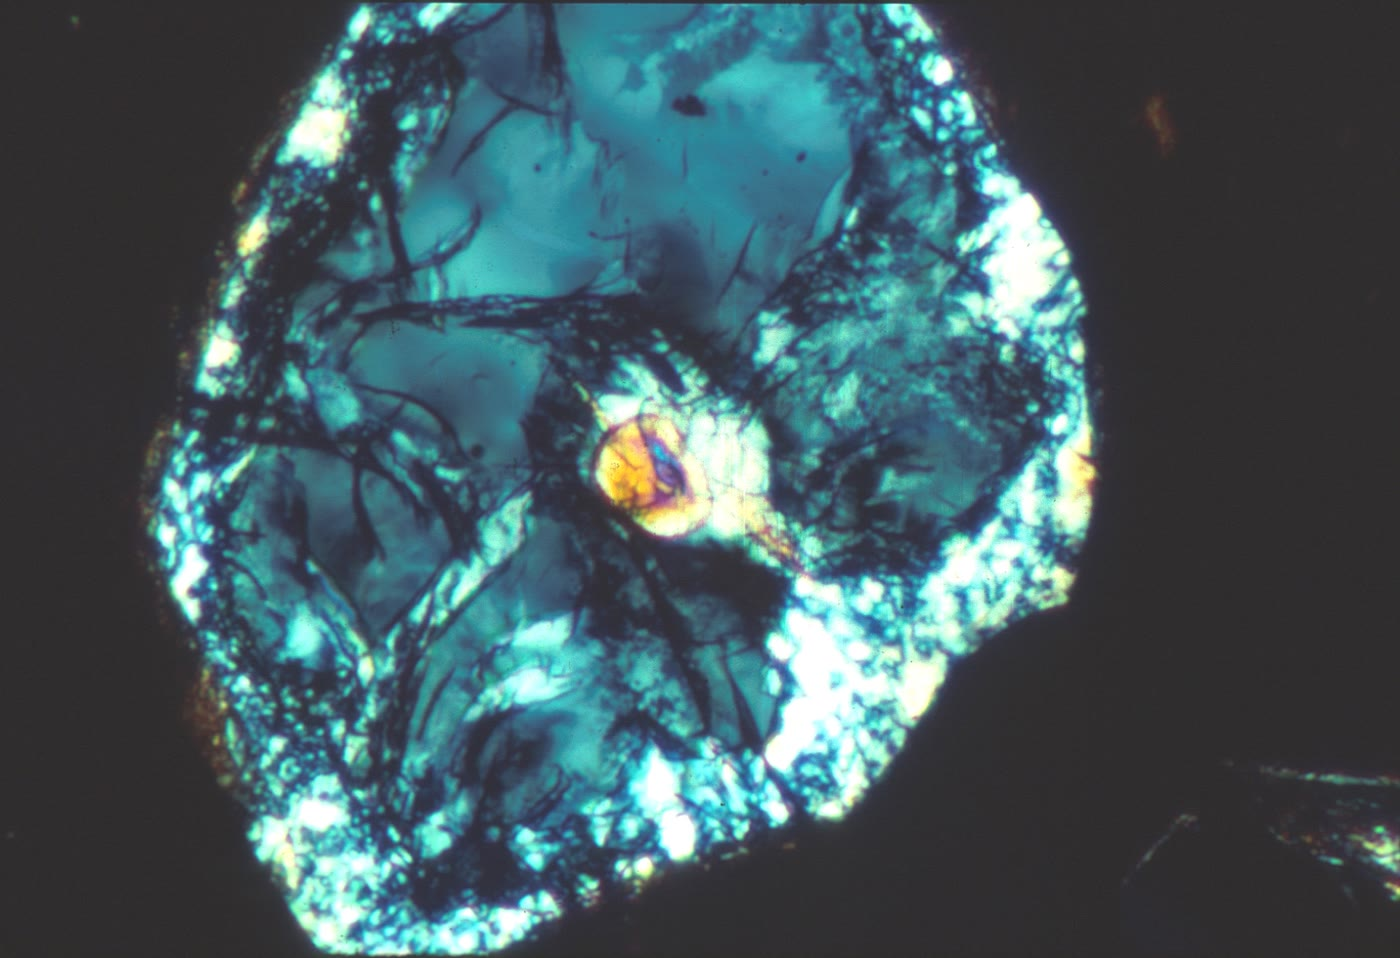
\includegraphics[width=0.62\linewidth]{images/book4/b2-11-coesite.jpg}
\par\smallskip{\small एक एक्लोजाइट में कोसाइट, लगभग \qty{1}{mm} चौड़ा, आड़े ध्रुवकों के बीच
एक पतली काट में: बड़ा केंद्रीय कण कोसाइट है, छोटे चमकीले कणों का घेरा
क्वार्ट्ज़ है जो दाब गिरने पर उससे उगा; केंद्र का छोटा रंगीन कण एक
पाइरॉक्सीन अंतर्वेश है। फ़ोटो: J.\,R. Smyth, CC BY-SA 1.0।}
\end{omfigure}

छह वर्ष बाद, उत्तरी कज़ाख़स्तान के कोकचेतव पुंजक के नाइसों, शिस्टों और
गार्नेट--पाइरॉक्सीन चट्टानों में औसतन \qty{12}{\micro m} के हीरे मिले, गार्नेट
और ज़िरकॉन में घिरे हुए, जिन्होंने उन्हें ग्रेफ़ाइट में बदलने से बचाया: वे \qty{40}{kbar}
या अधिक पर और 900 से \qty{1000}{\celsius} से ऊपर उगे। महाद्वीपीय भूपर्पटी, जितनी हल्की है, उसके बावजूद
सौ किलोमीटर से अधिक नीचे घसीटी जा सकती है।
% ledger: ss90:diamond

वह कैसे लौटती है, यह उसकी घड़ियाँ बताती हैं। आल्प्स की सबसे गहराई तक क्षेपित चट्टानों में,
क्रमिक चरणों पर काल-निर्धारित टाइटेनाइट दिखाता है कि एक कैल्क-सिलिकेट चट्टान लगभग
\qty{3.5}{GPa} पर $35.1 \pm \qty{0.9}{Ma}$ पर पहुँची, $1 \pm \qty{0.15}{GPa}$ पर $32.9 \pm
\qty{0.9}{Ma}$ पर थी, और 0.4 से \qty{0.5}{GPa} के निकट $31.8 \pm \qty{0.5}{Ma}$ पर। माध्य
\omterm{def:b2:pt-paths:exhumation}{उत्खनन-दरें}, पहले 3.4 फिर \qty{1.6}{cm.yr^{-1}}, प्लेटों की गतियों से मेल खाती हैं: चट्टानें
लगभग उतनी ही तेज़ी से लौटीं जितनी तेज़ी से नीचे गई थीं, अपरदन जितनी तेज़ी से उनका अनावरण कर सकता था उससे कहीं
अधिक तेज़ी से। लेखक उत्प्लावकता का सहारा लेते हैं, यानी हल्की भूपर्पटी का सघनतर प्रावार में से उठना, और
सामान्य भ्रंशन का, जो ऊपर की चट्टानों को पतला करता है।
% ledger: rh01:exhumation

\section{महासागर-तल कायांतरण}\label{sec:b2:pt-paths:ocean-floor}

\begin{definition}[महासागर-तल कायांतरण; सर्पेंटिनीकरण]\label{def:b2:pt-paths:ocean-floor}
\emph{महासागर-तल कायांतरण}\index{महासागर-तल कायांतरण} प्रसार केंद्रों के निकट
महासागरीय स्थलमंडल का क्षेत्रीय \omterm{def:b2:metamorphic-facies:metamorphism}{कायांतरण} है, जो खड़ी भूतापीय प्रवणताओं के अधीन
परिसंचारी गर्म जलीय तरलों द्वारा होता है; पुनःक्रिस्टलन सामान्यतः अपूर्ण होता है
और तापमान प्रायः गहराई के साथ बढ़ता है। \emph{सर्पेंटिनीकरण}\index{सर्पेंटिनीकरण}
ओलिवीन-समृद्ध चट्टानों का जलयोजन होकर सर्पेंटाइन बनना है।
\end{definition}
% ledger: scmr:types

किसी कटक-अक्ष के निकट युवा भूपर्पटी में खिंचा समुद्री जल गर्म होता है, चट्टानों से अभिक्रिया करता है और
फिर ऊपर उठता है। जिन बेसाल्टों से वह गुज़रता है वे तापमानों के एक विस्तृत परास में, अपूर्ण रूप से,
जलयोजित खनिजों में पुनःक्रिस्टलित होते हैं। जहाँ जल \omterm{def:b2:mantle-melting:peridotites}{पेरिडोटाइट} तक पहुँचता है, जैसे
उन धीमे कटकों पर जहाँ प्रावार-चट्टान समुद्र-तल तक ऊपर आती है और लॉस्ट सिटी जलतापीय क्षेत्र जैसे
स्रोतों को पोषित करती है (पुस्तक 3, स्नातक वर्ष 1), वहाँ ओलिवीन जल ग्रहण करता है:
\[
\ce{2 Mg2SiO4 + 3 H2O -> Mg3Si2O5(OH)4 + Mg(OH)2},
\]
फ़ॉर्स्टेराइट से सर्पेंटाइन और ब्रूसाइट। मोलर आयतन, फ़ॉर्स्टेराइट के लिए 43.65, सर्पेंटाइन के लिए 107.50
और ब्रूसाइट के लिए \qty{24.63}{cm^3.mol^{-1}}, दिखाते हैं कि इससे चट्टान पर क्या होता है:
\qty{87.30}{cm^3} ओलिवीन \qty{132.13}{cm^3} ठोस बन जाता है, \qty{51}{\percent}
अधिक, और घनत्व 3.22 से \qty{2.54}{g.cm^{-3}} तक गिर जाता है। चट्टान फूलती और
हल्की होती है, और जो जल उसने बाँधा है वह प्लेट के क्षेपित होने पर उसके साथ नीचे जाता है।
% ledger: scmr:types, rh95:serpentine, kelley:lost-city, dick:ultraslow

\begin{inthelab}[एक गार्नेट को पढ़ना]
\omterm{def:b2:pt-paths:paths}{P--T पथ} पढ़ने के लिए शैलिकीविद पहले किसी गार्नेट के केंद्र से होकर एक पतली काट काटता है,
क्योंकि केंद्र से हटी काट क्रोड को चूक जाती है। सूक्ष्मदर्शी के नीचे अंतर्वेशों
का मानचित्रण किया जाता है: क्वार्ट्ज़, बायोटाइट, प्लैजियोक्लेज़ या कायनाइट के छोटे कण जो गार्नेट के
उगते समय फँस गए, कभी-कभी ऐसी कतारों में संरेखित जो चट्टान के किसी पुराने पर्णन को सुरक्षित रखती हैं। फिर एक इलेक्ट्रॉन
माइक्रोप्रोब क्रोड से किनारे तक एक रेखा के अनुदिश संघटन मापता है, और
मैग्नीशियम, लोहे, कैल्सियम और मैंगनीज़ का एक मानचित्र वृद्धि-मंडल दिखाता है। हर मंडल को
उन खनिजों के साथ जोड़ा जाता है जो उसके साथ उगे: क्रोड के लिए अंतर्वेश, किनारे के लिए संपर्क में
स्थित आधात्री। हर युग्म पर तापमापी और दाबमापी लगाए जाते हैं, और जहाँ कोई
खनिज अनुमति दे वहाँ मंडलों का काल-निर्धारण किया जाता है। \Cref{ch:b2:field-lab-methods-2} उपकरणों का वर्णन करता है।
\end{inthelab}

\begin{omfigure}
\centering
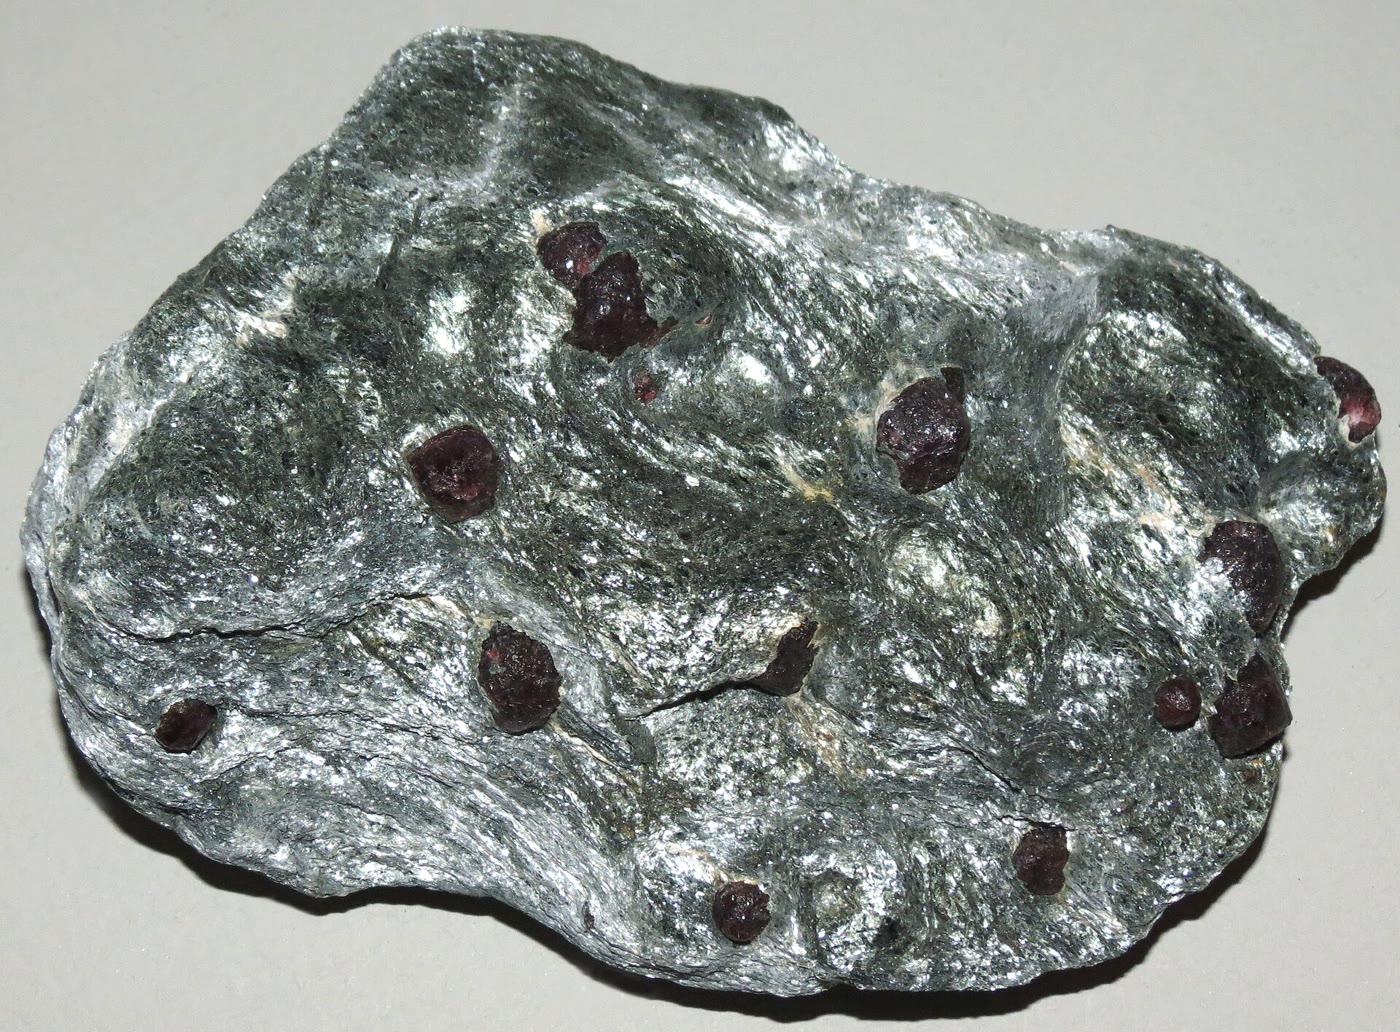
\includegraphics[width=0.62\linewidth]{images/book4/b2-11-garnet-schist.jpg}
\par\smallskip{\small एक गार्नेट शिस्ट: अभ्रकों की पर्णित आधात्री में उगे गहरे लाल गार्नेट
क्रिस्टल। हर गार्नेट क्रोड से किनारे तक चट्टान के पथ का
अभिलेख रख सकता है। फ़ोटो: James St.~John, CC BY 2.0।}
\end{omfigure}

\section{अभ्यास}

\begin{exercise}[$\star$]\label{exo:b2:pt-paths:1}
एक ही पंकाश्म शैलसमूह के छह नमूने, जो एक सड़क के किनारे एकत्र किए गए, ये रखते हैं: (A) क्लोराइट,
मस्कोवाइट, क्वार्ट्ज़; (B) बायोटाइट, क्लोराइट, मस्कोवाइट, क्वार्ट्ज़; (C) गार्नेट, बायोटाइट,
मस्कोवाइट, क्वार्ट्ज़; (D) स्टॉरोलाइट, गार्नेट, बायोटाइट, मस्कोवाइट, क्वार्ट्ज़; (E) कायनाइट,
स्टॉरोलाइट, बायोटाइट, मस्कोवाइट, क्वार्ट्ज़; (F) सिलिमेनाइट, बायोटाइट, मस्कोवाइट, क्वार्ट्ज़।
(क) हर एक किस \omterm{def:b2:pt-paths:barrovian}{बैरोवियन मंडल} में स्थित है? (ख) सड़क कितनी समश्रेणी-रेखाएँ पार करती है, और
कौन-सी? (ग) \omterm{def:b2:pt-paths:barrovian}{कायांतरी क्षेत्र-प्रवणता} खींचने के लिए समश्रेणी-रेखाओं को जानना पर्याप्त क्यों
नहीं है?
\end{exercise}
% ledger: iugs:barrow

\begin{exercise}[$\star$]\label{exo:b2:pt-paths:2}
एक गार्नेट में $X_{\text{Mg}} = 0.10$ और $X_{\text{Fe}} = 0.80$ है, उसके बगल के बायोटाइट में
$X_{\text{Mg}} = 0.45$ और $X_{\text{Fe}} = 0.50$। (क) $K_D$ और $\ln K_D$ परिकलित कीजिए।
(ख) इस अध्याय के अंशांकन से \qty{5}{kbar} पर और
\qty{7}{kbar} पर तापमान परिकलित कीजिए। (ग) परिणाम तापमान का मापक है या दाब का?
\end{exercise}
% ledger: h97:ideal, h97:fs-reaction

\begin{exercise}[$\star$]\label{exo:b2:pt-paths:3}
एक \omterm{def:b2:metamorphic-facies:protoliths}{मेटापेलाइट} \qty{580}{\celsius} और \qty{6.0}{kbar} देता है। (क) माध्य
घनत्व \qty{2800}{kg.m^{-3}} की चट्टानों के नीचे ($g = \qty{9.81}{m.s^{-2}}$), वह कितनी गहराई पर था? (ख) सतह पर
\qty{10}{\celsius} से इससे किस तापमान-प्रवणता का संकेत मिलता है? (ग) प्रायोगिक
कायनाइट $=$ सिलिमेनाइट रेखा \qty{3.67}{kbar} से होकर जाती है,
\qty{500}{\celsius} पर, और \qty{5.77}{kbar} से, \qty{600}{\celsius} पर: चट्टान में कौन-सा ऐलुमिनोसिलिकेट
होना चाहिए?
\end{exercise}
% ledger: hm93:table11

\begin{exercise}[$\star$]\label{exo:b2:pt-paths:4}
इस अध्याय में लिखे फ़ॉर्स्टेराइट के \omterm{def:b2:pt-paths:ocean-floor}{सर्पेंटिनीकरण} के लिए: (क) जाँचिए कि
समीकरण द्रव्यमान में संतुलित है, मोलर द्रव्यमानों 140.693 (फ़ॉर्स्टेराइट), 18.015 (जल),
277.112 (सर्पेंटाइन) और \qty{58.320}{g.mol^{-1}} (ब्रूसाइट) के साथ; (ख) ठोसों के
आयतन में परिवर्तन परिकलित कीजिए; (ग) ओलिवीन के और उत्पादों के घनत्व परिकलित कीजिए।
(घ) यह परिवर्तन समुद्र-तल के नीचे किसी सर्पेंटिनीकृत \omterm{def:b2:mantle-melting:peridotites}{पेरिडोटाइट} पर क्या प्रभाव डालता है?
\end{exercise}
% ledger: rh95:serpentine

\begin{exercise}[$\star\star$]\label{exo:b2:pt-paths:5}
\qty{2.07}{kbar} पर हुए चार प्रयोगों से तापमापी का अंशांकन कीजिए: $\ln K_D =
-1.157$ और $-1.255$, \qty{799}{\celsius} पर, $-1.738$ और $-1.826$, \qty{550}{\celsius} पर।
(क) हर युग्म का औसत लीजिए और दोनों माध्यों से होकर जाने वाली रेखा $\ln K_D = a/T + b$ ज्ञात कीजिए।
(ख) $\Delta_r H$ और $\Delta_r S$ निगमित कीजिए, $\Delta_r V = \qty{0.311}{J.bar^{-1}}$ के साथ।
(ग) आपका अंशांकन और अध्याय का अंशांकन
\qty{5}{kbar} पर $K_D = 0.18$, $0.10$ और $0.30$ के लिए जो तापमान देते हैं, उनकी तुलना कीजिए। किसी
अंशांकन के बहिर्वेशन के बारे में आप क्या निष्कर्ष निकालते हैं?
\end{exercise}
% ledger: h97:fs-data, h97:ideal

\begin{exercise}[$\star\star$]\label{exo:b2:pt-paths:6}
(क) \qty{298}{K} पर मोलर आयतनों (ऐल्मंडीन 115.32, पाइरोप 113.12, ऐनाइट
154.30, फ़्लोगोपाइट 149.65, ग्रॉस्युलर 125.28, एनॉर्थाइट 100.79, कायनाइट 44.15, क्वार्ट्ज़
\qty{22.69}{cm^3.mol^{-1}}) से विनिमय और GASP
अभिक्रिया का $\Delta_r V$ परिकलित कीजिए, और अंशांकनों द्वारा प्रयुक्त मानों, \num{0.311} और
\qty{-6.21}{J.bar^{-1}}, से तुलना कीजिए। (ख) $K_D = 0.18$ के लिए
\qty{1}{kbar} की त्रुटि तापमान को कितने केल्विन खिसकाती है? (ग) 
$X_{\text{Ca}}/X_{\text{एनॉ}} = 0.20$ वाली चट्टान की GASP रेखा के अनुदिश, \qty{17}{K} की त्रुटि
दाब को कितने बार खिसकाती है?
\end{exercise}
% ledger: rh95:gb-gasp, rh95:al2sio5, h97:fs-reaction, kn88:gasp

\begin{exercise}[$\star\star$]\label{exo:b2:pt-paths:7}
\qty{600}{\celsius} पर एक गार्नेट में $X_{\text{Ca}} = 0.08$ है और उसके बगल के प्लैजियोक्लेज़ में
$X_{\text{एनॉ}} = 0.30$। (क) GASP दाब परिकलित कीजिए। (ख) इसे $X_{\text{एनॉ}} =
0.35$ के साथ फिर से कीजिए। (ग) \qty{2800}{kg.m^{-3}} के माध्य घनत्व के लिए चट्टान कितनी गहराई पर थी?
\end{exercise}
% ledger: kn88:gasp

\begin{exercise}[$\star\star$]\label{exo:b2:pt-paths:8}
आल्प्स की सबसे गहराई तक क्षेपित चट्टानों की टाइटेनाइट आयु का उपयोग कीजिए: लगभग \qty{3.5}{GPa},
$35.1 \pm \qty{0.9}{Ma}$ पर, \qty{1.0}{GPa}, $32.9 \pm \qty{0.9}{Ma}$ पर, \qty{0.45}{GPa},
$31.8 \pm \qty{0.5}{Ma}$ पर। (क) \qty{3000}{kg.m^{-3}} के माध्य घनत्व के साथ दाबों को
गहराइयों में बदलिए। (ख) दोनों माध्य \omterm{def:b2:pt-paths:exhumation}{उत्खनन-दरें} परिकलित कीजिए और उनकी तुलना
प्रकाशित 3.4 और \qty{1.6}{cm.yr^{-1}} से कीजिए। (ग) पहले समय-अंतराल की
अनिश्चितता क्या है, और वह दरों के किस परास की अनुमति देती है? (घ) मोटा होने वाले मॉडल की
अपरदन-दर, \qty{0.5}{mm.yr^{-1}}, से तुलना कीजिए।
\end{exercise}
% ledger: rh01:exhumation

\begin{exercise}[$\star\star$]\label{exo:b2:pt-paths:9}
\qty{5}{kbar} पर $K_D = 0.18$ के लिए, (क) प्रतिज्ञप्ति से $\partial T/\partial\ln K_D$ और
$\partial T/\partial P$ परिकलित कीजिए; (ख) $\sigma_{\ln K_D} = 0.05$ ($K_D$ पर
\qty{5}{\percent} की त्रुटि) और $\sigma_P = \qty{1}{kbar}$ के साथ $\sigma_T$ परिकलित कीजिए।
(ग) कौन-सी त्रुटि प्रभावी है? सबसे अच्छे अंशांकनों के लिए दावा की गई \qty{25}{\celsius} की अनिश्चितता से
तुलना कीजिए।
\end{exercise}
% ledger: h97:ideal

\begin{exercise}[$\star\star\star$]\label{exo:b2:pt-paths:10}
एक गार्नेट-किनारे में $X_{\text{Mg}} = 0.10$, $X_{\text{Fe}} = 0.75$, $X_{\text{Ca}} = 0.07$ है;
आधात्री के बायोटाइट में $X_{\text{Mg}} = 0.42$, $X_{\text{Fe}} = 0.52$; प्लैजियोक्लेज़ में
$X_{\text{एनॉ}} = 0.25$। (क) \qty{6}{kbar} से शुरू करके इस अध्याय की विधि लागू कीजिए,
जब तक तापमान \qty{1}{K} से कम न बदले। (ख) चट्टान में कौन-सा ऐलुमिनोसिलिकेट
होना चाहिए (\cref{exo:b2:pt-paths:3} की प्रायोगिक रेखा का उपयोग कीजिए)? (ग) दाबमापी को
वास्तव में उपस्थित ऐलुमिनोसिलिकेट का ही उपयोग क्यों करना चाहिए?
\end{exercise}
% ledger: h97:ideal, kn88:gasp, hm93:table11

\begin{exercise}[$\star\star\star$]\label{exo:b2:pt-paths:11}
$\kappa = \qty{1e-6}{m^2.s^{-1}}$ के साथ: (क) $L = \qty{35}{km}$ और
$L = \qty{70}{km}$ के लिए प्रतिज्ञप्ति का शिथिलन-काल परिकलित कीजिए। (ख) मॉडल
70 मिलियन वर्षों में \qty{35}{km} का अपरदन करता है; उस समय की तुलना (क) के दोनों समयों से कीजिए। (ग)
इन समयों से समझाइए कि मॉडल की चट्टान अपने दाब-शिखर के बाद अपने तापीय शिखर पर
क्यों पहुँचती है। (घ) यदि अपरदन दस गुना तेज़ होता, तो पथ में क्या बदलता?
\end{exercise}
% ledger: delaney:conductivity, et84:ptt

\begin{exercise}[$\star\star\star$]\label{exo:b2:pt-paths:12}
\qty{2800}{kg.m^{-3}} घनत्व वाली \qty{35}{km} मोटी एक भूपर्पटी लीजिए, जो
\qty{3300}{kg.m^{-3}} के प्रावार के ऊपर है। (क) किस गहराई पर दाब \qty{28}{kbar} तक पहुँचता है, जो
डोरा माइरा कोसाइट के लिए न्यूनतम है? (ख) और \qty{40}{kbar}, कोकचेतव हीरों के लिए?
(ग) (क) की गहराई पर \qty{700}{\celsius} किस माध्य प्रवणता का संकेत देता है, और वह किस
श्रेणी में आती है? (घ) \qty{3.4}{cm.yr^{-1}} पर, (क) की गहराई से
\qty{35}{km} तक की चढ़ाई में कितना समय लगता है?
\end{exercise}
% ledger: chopin84:coesite, ss90:diamond, rh01:exhumation

\section{समस्या: एक गार्नेट की यात्रा}

\begin{problem}[{सप्ताहांत समस्या --- एक शिस्ट की तापदाबमिति, पथ और
उत्खनन-दर}]
\label{pb:b2:pt-paths:1}
एक कायनाइट--गार्नेट--बायोटाइट शिस्ट में क्रोड और किनारे वाले गार्नेट हैं। क्रोड
बायोटाइट, प्लैजियोक्लेज़ और कायनाइट को घेरे हुए है; किनारा आधात्री के बायोटाइट और प्लैजियोक्लेज़ को
छूता है। गार्नेटों के चारों ओर कुछ कायनाइट सिलिमेनाइट से प्रतिस्थापित है, और
गार्नेटों के किनारों पर कुछ क्लोराइट उगा है। विश्लेषण ये हैं:
\begin{center}
\small
\begin{tabular}{@{}lccc@{}}
\hline
 & $X_{\text{Mg}}$ & $X_{\text{Fe}}$ & $X_{\text{Ca}}$ या $X_{\text{एनॉ}}$\\
\hline
गार्नेट क्रोड & 0.080 & 0.760 & 0.050\\
क्रोड में अंतर्वेशित बायोटाइट & 0.40 & 0.58 & ---\\
क्रोड में अंतर्वेशित प्लैजियोक्लेज़ & --- & --- & 0.25\\
गार्नेट किनारा & 0.120 & 0.720 & 0.060\\
आधात्री बायोटाइट & 0.46 & 0.53 & ---\\
आधात्री प्लैजियोक्लेज़ & --- & --- & 0.28\\
\hline
\end{tabular}
\end{center}
इस अध्याय के गार्नेट--बायोटाइट तापमापी और GASP दाबमापी (आदर्श मिश्रण) का उपयोग कीजिए,
$R = \qty{8.314}{J.mol^{-1}.K^{-1}}$, $g = \qty{9.81}{m.s^{-2}}$, चट्टान के ऊपर
\qty{2800}{kg.m^{-3}} का माध्य घनत्व, और हर अनुपात को चार दशमलव तक पूर्णांकित कीजिए।

\noindent\textbf{भाग I --- तापमान।}
\begin{enumerate}
\item गार्नेट क्रोड में और अंतर्वेशित
बायोटाइट में $X_{\text{Mg}}/X_{\text{Fe}}$ परिकलित कीजिए, फिर क्रोड के लिए $K_D$ और $\ln K_D$।
\item किनारे और आधात्री बायोटाइट के लिए भी यही कीजिए।
\item \qty{6}{kbar} पर क्रोड का तापमान परिकलित कीजिए।
\item \qty{6}{kbar} पर किनारे का तापमान परिकलित कीजिए।
\item \qty{1}{kbar} की त्रुटि इन तापमानों को कितने केल्विन बदलेगी?
\item क्रोड को अंतर्वेशित बायोटाइट के साथ, और किनारे को आधात्री
बायोटाइट के साथ क्यों जोड़ा जाता है?
\end{enumerate}

\noindent\textbf{भाग II --- दाब।}
\begin{enumerate}[resume]
\item प्रश्न~3 और~4 के दोनों तापमानों पर GASP अभिक्रिया का अंत्य-सदस्य दाब $P_0$
परिकलित कीजिए।
\item प्रश्न~3 के तापमान पर क्रोड का GASP दाब परिकलित कीजिए।
\item प्रश्न~4 के तापमान पर किनारे का GASP दाब परिकलित कीजिए।
\item प्रश्न~9 के दाब पर किनारे का तापमान फिर से परिकलित कीजिए, फिर उस तापमान पर उसका
दाब, और एक बार फिर तापमान। किनारे का तापमान
और दाब बताइए।
\item क्रोड के लिए भी एक बार यही कीजिए। वह इतना कम क्यों बदलता है?
\item क्रोड और किनारे के दाबों को गहराइयों में बदलिए।
\item प्रायोगिक कायनाइट $=$ सिलिमेनाइट रेखा 3.67, 5.77 और
\qty{7.86}{kbar} से होकर जाती है, 500, 600 और \qty{700}{\celsius} पर। क्रोड के उगते समय कौन-सा ऐलुमिनोसिलिकेट स्थायी था,
और किनारे के उगते समय? क्या क्रोड का कायनाइट संगत है?
\end{enumerate}

\noindent\textbf{भाग III --- पथ।}
\begin{enumerate}[resume]
\item क्रोड और किनारे के बीच तापमान और दाब कितने बदले?
गार्नेट \omterm{def:b2:pt-paths:paths}{प्रगामी पथ} पर उग रहा था या प्रतिगामी पर?
\item गार्नेटों के चारों ओर सिलिमेनाइट कायनाइट का स्थान लेता है। किनारे के तापमान पर,
ऐसा होने के लिए चट्टान को किस दाब से नीचे गुज़रना पड़ा होगा? किनारा उगने के बाद चट्टान ने
क्या किया?
\item गार्नेटों के किनारों पर क्लोराइट उगता है। वह पथ के किस भाग को अंकित करता है?
\item पथ खींचिए: क्रोड, किनारा, सिलिमेनाइट, क्लोराइट। वह दक्षिणावर्त है या वामावर्त?
कौन-सा शिखर पहले आया?
\item इस अध्याय का मोटा होने वाला मॉडल अपनी चट्टान को \qty{593}{\celsius} के तापीय शिखर पर
\qty{7.8}{kbar} पर लाता है। क्या शिस्ट का पथ उसी प्रकार का है?
\end{enumerate}

\noindent\textbf{भाग IV --- कितनी तेज़ी से।}
\begin{enumerate}[resume]
\item गार्नेट-किनारा $412.0 \pm \qty{1.5}{Ma}$ की समेरियम--नियोडिमियम आयु देता है, जिसे
शिखर की आयु माना जाता है; आधात्री का एक मस्कोवाइट $398.0 \pm
\qty{1.0}{Ma}$ की आर्गन आयु देता है, वह समय जब चट्टान ठंडी होकर \qty{405}{\celsius} से गुज़री। उनके बीच
माध्य शीतलन-दर परिकलित कीजिए।
\item \qty{405}{\celsius} का अवरोध-तापमान
\qty{10}{\celsius} प्रति मिलियन वर्ष के शीतलन को मानकर चलता है। क्या प्रश्न~19 की दर किसी उच्चतर या
निम्नतर मान की माँग करती है, और क्यों?
\item \qty{398}{Ma} पर, सतह पर \qty{10}{\celsius} से शुरू होने वाला \qty{30}{\celsius\per\km} का जियोथर्म
लीजिए। मस्कोवाइट किस गहराई पर बंद हुआ?
\item शिखर और मस्कोवाइट के बंद होने के बीच चट्टान कितनी ऊपर उठी?
\item समय-अंतराल की अनिश्चितता क्या है?
\item शिखर से मस्कोवाइट के बंद होने तक की माध्य \omterm{def:b2:pt-paths:exhumation}{उत्खनन-दर} परिकलित कीजिए,
मिलीमीटर प्रति वर्ष में और दशमांश तक पूर्णांकित: यह इस समस्या की मुख्य संख्या है।
\end{enumerate}
\end{problem}
% ledger: h97:ideal, h97:fs-reaction, kn88:gasp, hm93:table11, h09:muscovite, scmr:ptt, et84:ptt
